\section{WordNet}
\begin{frame}
\frametitle{WordNet}

\includegraphics[scale=0.35]{img/wordnet_logo.png}
\begin{itemize}
\item development started 1985
\item lexical database for English language
\item covers most English nouns, verbs, adjectives, adverbs
\item used in many applications (retrieval, translation)
\item two kinds of semantic relations
\end{itemize}
% which means it labels concepts to words
\end{frame}

\begin{frame}
\begin{itemize}
\frametitle{Synsets - Lexical (word-word) relation}
\item words are grouped into synonym sets - synsets
\item sysnsets are the basic unit of meaning
\item 120,000 synsets
\item Synonym, Antonymy, Gradation
\end{itemize}
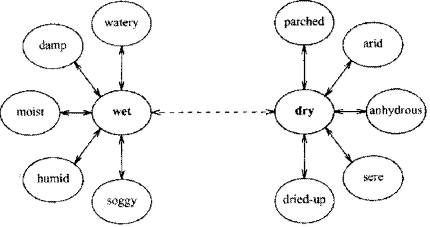
\includegraphics[scale=0.55]{img/wordnet-syn.png}
% Gradation in this context means it's related to all comparative words, for example wet, wetter, the wettest
\end{frame}

\begin{frame}
\begin{itemize}
\frametitle{Homonyms}
\item Homonyms are represented in several Synsets
\end{itemize}
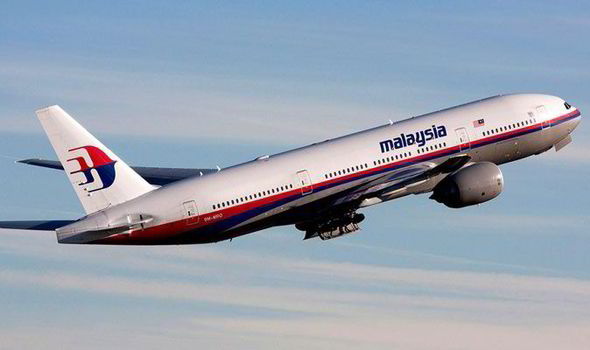
\includegraphics[scale=0.25]{img/plane2.jpg}
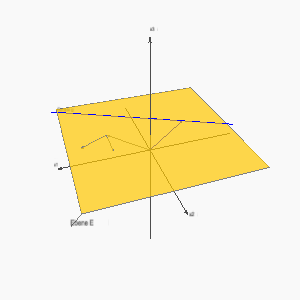
\includegraphics[scale=0.29]{img/wordnet_plane1.png}
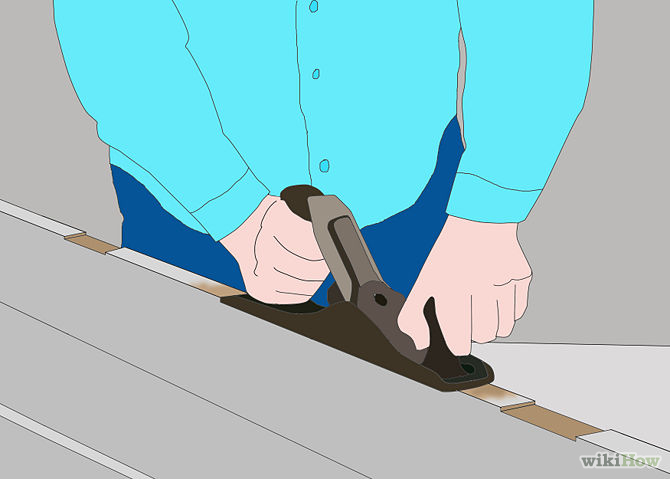
\includegraphics[scale=0.18]{img/plane3.jpg}
\end{frame}

\begin{frame}
\begin{minipage}{0.40\textwidth}
\begin{itemize}
\frametitle{Linking between Synsets - Conceptual (concept-concept) relation}
\item Synsets are linked by
\begin{itemize}
\item Hypernymy / Hyponymy
\item Meronymy / Holonymy 
\item Entailment 
\item Troponymy
\end{itemize}
\end{itemize}
\end{minipage}
\begin{minipage}{0.5\textwidth}
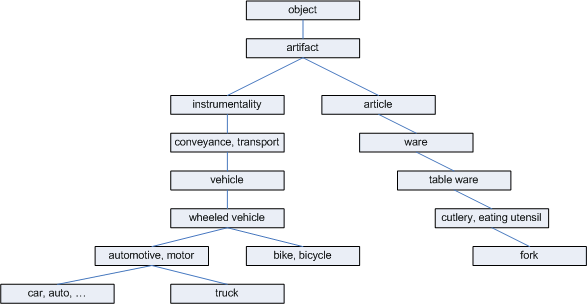
\includegraphics[scale=0.33]{img/wordnet_hyponym.png}
\end{minipage}
\end{frame}

\begin{frame}
\frametitle{Hypernym / Hyponym}
\begin{minipage}{0.5\textwidth}
\begin{itemize}
\item A truck (Hyponym) is a kind of car (Hypernym)
\item denotes more or less general concepts
\item transitive
\item experiments indicate knowledge about concepts is stored at superordinate (Hypernym) nodes and inherited downward
\end{itemize}
\end{minipage}
\begin{minipage}{0.4\textwidth}
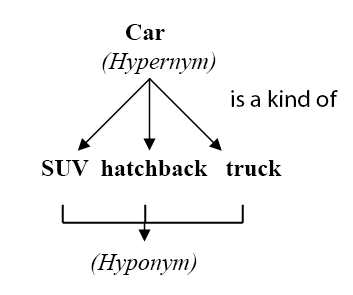
\includegraphics[scale=0.33]{img/wordnet_hyp.png}
\end{minipage}
% This relation is transitive so if for example a car is a kind of vehicle then a truck is also a kind of vehicle. Reaction time word association experiments with humans suggest that knowledge is stored in the brain at superordinate nodes and inherited downward. 
\end{frame}

\begin{frame}
\frametitle{Meronym / Holonym (part/whole)}
\begin{minipage}{0.5\textwidth}
\begin{itemize}
\item The engine (Hyponym) is a part of a car (Hypernym)
\item denotes more or less general concepts
\item inheritance
\item 3 kinds of meronomy
\begin{itemize}
\item proper parts
\item substance
\item groups/members
\end{itemize}
\end{itemize}
\end{minipage}
\begin{minipage}{0.4\textwidth}
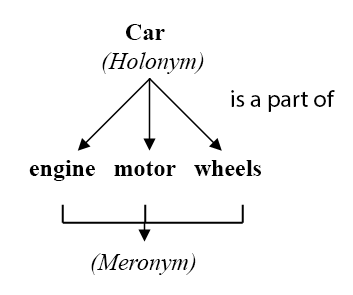
\includegraphics[scale=0.33]{img/wordnet_mer.png}
\end{minipage}
% An example for the inheritance would be that is an engine has spark plugs and an enginge is part of a car, then a car also has spark plugs. 
% WordNet distinguishes between 3 different kinds of Meronomy. First there are proper parts, which are seperable, like in the example: car - engine, or motor engine. Then there is are substances such as oxygen which is a part of air and water and members of groups like professor and faculty.
\end{frame}

\begin{frame}
\frametitle{Semantic Relations between Verbs}
\begin{itemize}
\item apart from Homonyms
\begin{itemize}
\item Troponym:\\
the verb Y is a troponym of the verb X if the activity Y is doing X in some manner (lisp- talk)
\item Entailment:\\
the verb Y is entailed by X if by doing X you must be doing Y (sleep - snore)
\end{itemize}
\end{itemize}
%the verb Y is a troponym of the verb X if the activity Y is doing X in some manner (to lisp is a troponym of to talk)
%the verb Y is entailed by X if by doing X you must be doing Y (to sleep is entailed by to snore)
\end{frame}

\begin{frame}
\frametitle{Problems and Limitations}
\begin{itemize}
\item doesn't contain etymology, pronunciation or irregular verbs
\item hard to modify or maintain
\item no special domain vocabulary
\item granularity
\end{itemize}
\end{frame}


\begin{frame}
\frametitle{Demo}
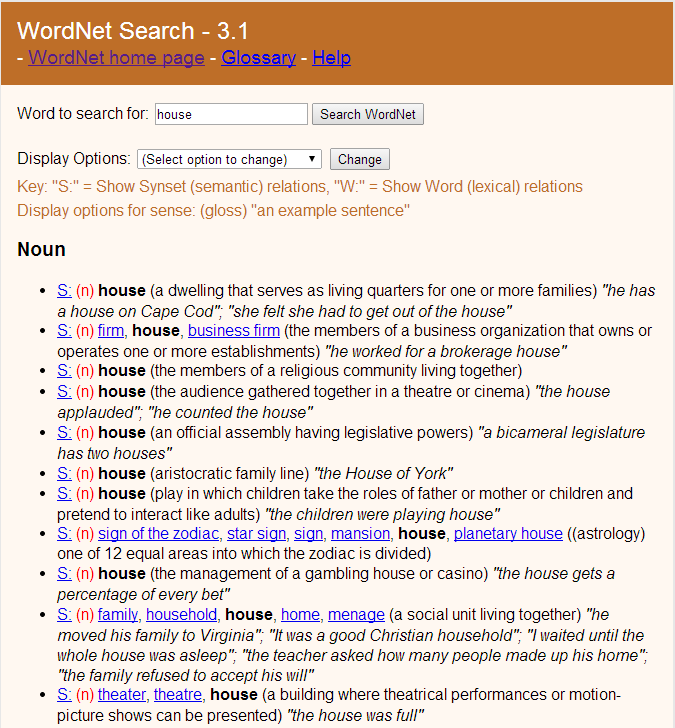
\includegraphics[scale=0.29]{img/wordnet_demo.png}\\
http://wordnetweb.princeton.edu/perl/webwn
\end{frame}

\begin{frame}
\frametitle{Demo - Python + TextBlob}
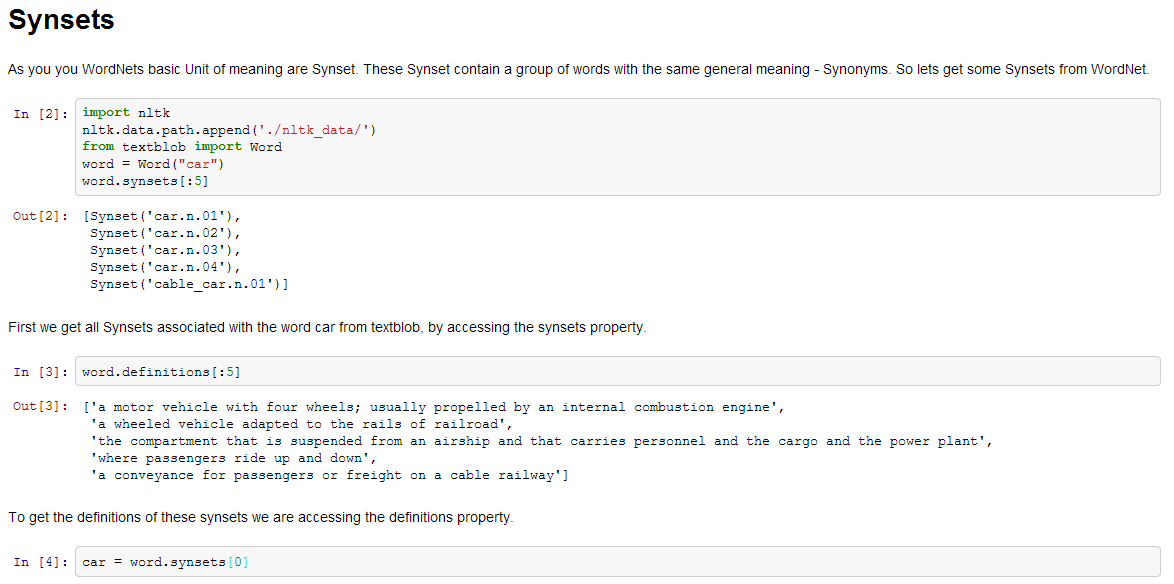
\includegraphics[scale=0.29]{img/wordnet_ip1.PNG}\\
\end{frame}

\begin{frame}
\frametitle{Demo - Python + TextBlob}
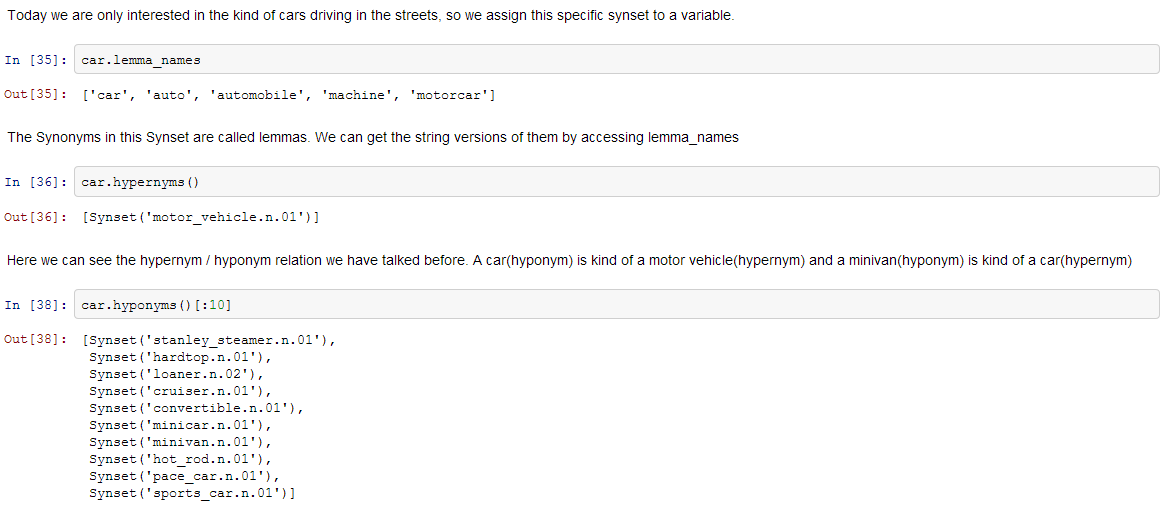
\includegraphics[scale=0.29]{img/wordnet_ip2.PNG}\\
\end{frame}

\begin{frame}
\frametitle{Demo - Python + TextBlob}
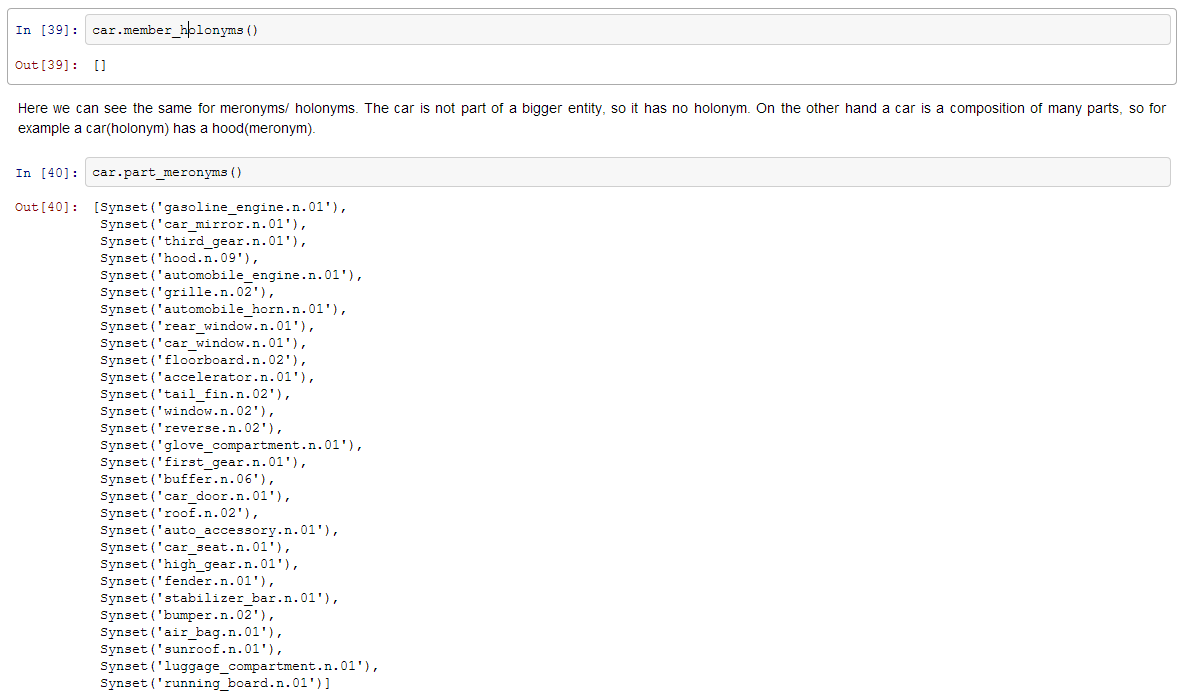
\includegraphics[scale=0.29]{img/wordnet_ip3.PNG}\\
\end{frame}

\begin{frame}
\frametitle{Demo - Python + TextBlob}
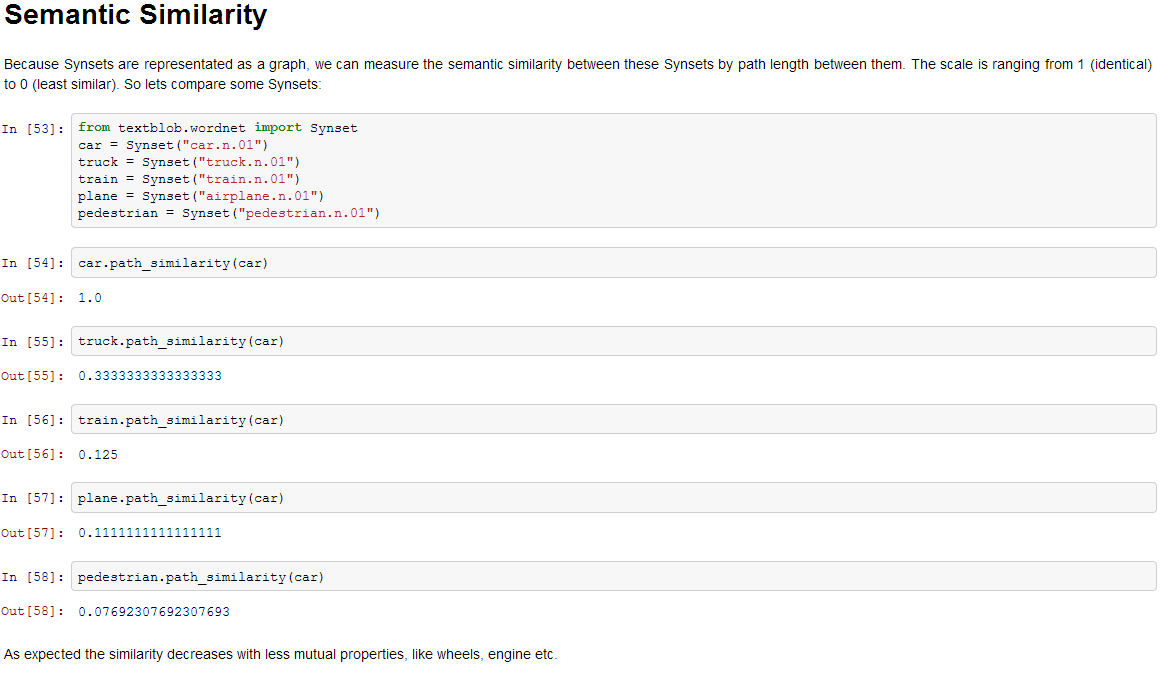
\includegraphics[scale=0.29]{img/wordnet_ip4.PNG}\\
\end{frame}

\begin{frame}
\frametitle{Application}
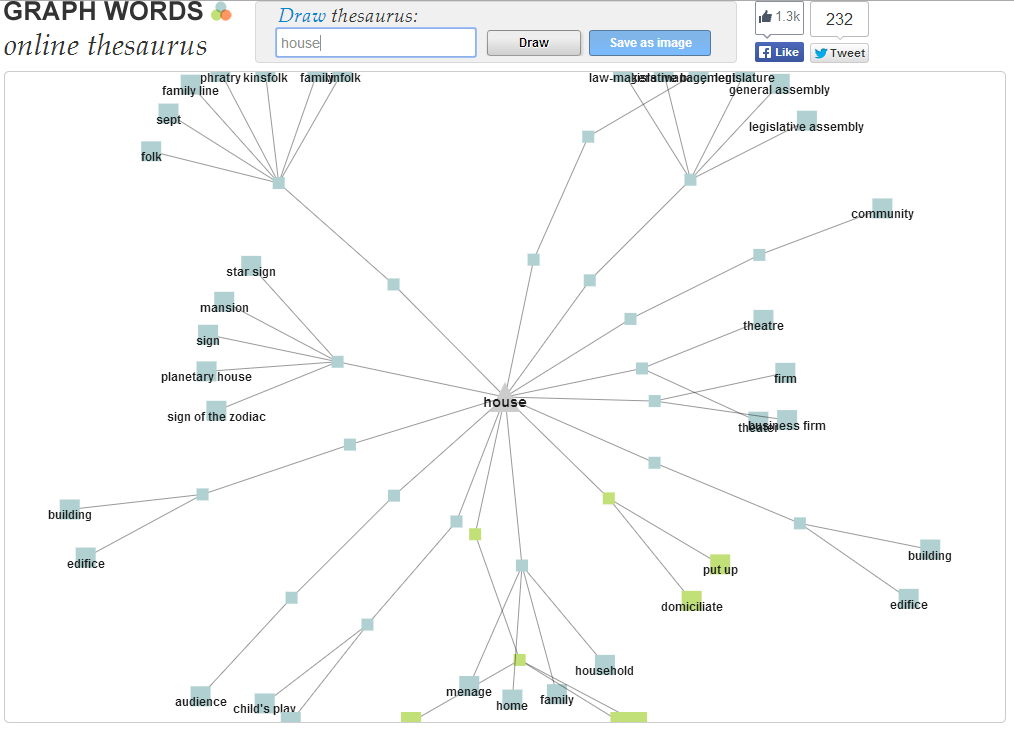
\includegraphics[scale=0.29]{img/wordnet_app.png}\\
http://graphwords.com/
\end{frame}

\begin{frame}
\frametitle{When to use Wordnet}
Since WordNet is a lexical Database it has different UseCases:
\begin{itemize}
\item taxonomic backbone
\item information retrieval
\item translation
\item Thesaurus
\end{itemize}
\end{frame}

\begin{frame}
\frametitle{Other WordNets}
There are many other WordNets for other languages
\begin{itemize}
\item Universal WordNet
\begin{itemize}
\item 1.5 million words
\item 200 languages
\item based on WordNet
\item MENTA integration\\
$\rightarrow$15 million words and names
\end{itemize}
\item GermaNet
\begin{itemize}
\item exclusive for German language
\item 93,000 synsets
\item 120,000 lexical units
\item for academics free
\end{itemize}
\item EuroWordNet
\begin{itemize}
\item Dutch, Italian, Spanish, German, French, Czech and Estonian
\item 200,000 synsets
\item not free
\item needs to be licensed
\end{itemize}
\end{itemize}
\end{frame}